% PROSZĘ KOMPILOWAĆ TEN DOKUMENT ZA POMOCĄ SILNIKA XELATEX
% W PRZECIWNYM RAZIE NALEŻY USUNĄĆ PAKIET fontspec ORAZ USTAWIENIA FONTU
% Z PLIKU styles/prez_wmini_pl.sty (PIERWSZE TRZY LINIJKI)
% W PRZYPADKU BRAKU FONTU Adagio Slab NALEŻY ZGŁOSIĆ SIĘ DO BIP PW O JEGO UDOSTĘPNIENIE,
% ZAŁADOWAĆ INNY KRÓJ CZCIONKI LUB ZAKOMENTOWAĆ/USUNĄĆ USTAWIENIA FONTU

\documentclass[aspectratio=169]{beamer}  %  , handout

\graphicspath{{images/}}

\usepackage{amssymb}
\usepackage{amsmath}
\usepackage{polski}
\usepackage[utf8]{inputenc}
\usepackage{hyperref}
\usepackage{blindtext}
\usepackage{multicol}
\usepackage{multirow}
\usepackage{wrapfig}
\usepackage{float}
\usepackage{enumitem}
\usepackage{xfrac}
\usepackage{caption}
\usepackage{subcaption}
\usepackage{booktabs}
\usepackage{wasysym}
\usepackage{xcolor}
\usepackage{pdfpages}
\usepackage{fontspec}
\usepackage{comment}
\usepackage{tocloft}
\usepackage{listings}
\usepackage{times}
\usepackage{amsmath}
\usepackage{bm}
\lstset{basicstyle=\ttfamily, columns=fullflexible}

\usepackage{caption, copyrightbox}
\captionsetup{justification=centering, labelfont=sc, labelsep=endash}

\usepackage{regexpatch}
\usepackage[os=mac]{menukeys}
\renewmenumacro{\keys}[+]{shadowedroundedkeys}
\renewmenumacro{\menu}[>]{angularmenus}
\xpatchcmd*{\SPACE}{2em}{1em}{}{}

\definecolor{quotationcolour}{HTML}{F0F0F0}
\definecolor{quotationmarkcolour}{HTML}{1F3F81}

% Double-line for start and end of epigraph.
\newcommand{\epiline}{\hrule \vskip -.2em \hrule}
% Massively humongous opening quotation mark.
\newcommand{\hugequote}{%
  \fontsize{42}{48}\selectfont \color{quotationmarkcolour} \textbf{``}
  \vskip -.5em
}

% Beautify quotations.
\newcommand{\epigraph}[2]{%
  \bigskip
  \begin{center}
  \colorbox{quotationcolour}{%
    \parbox{.80\textwidth}{%
    \epiline \vskip 1em {\hugequote} \vskip -.5em
    \parindent 2.2em
    #1\vspace{-.25cm}\begin{flushright}\textsc{#2}\end{flushright}
    \epiline
    }
  }
  \end{center}
  \bigskip
}

\setmainfont{Verdana}

\addtolength{\cftsecnumwidth}{5pt}
\addtolength{\cftsubsecnumwidth}{5pt}
\addtolength{\cftsubsubsecnumwidth}{5pt}
	
\usepackage{color, colortbl}
\definecolor{Gray}{gray}{0.9}

\definecolor{mGreen}{rgb}{0,0.6,0}
\definecolor{mGray}{rgb}{0.5,0.5,0.5}
\definecolor{mPurple}{rgb}{0.58,0,0.82}
\definecolor{backgroundColour}{rgb}{0.95,0.95,0.92}

\lstdefinestyle{CStyle}{
    backgroundcolor=\color{backgroundColour},   
    commentstyle=\color{mGreen},
    keywordstyle=\color{magenta},
    numberstyle=\tiny\color{mGray},
    stringstyle=\color{mPurple},
    basicstyle=\footnotesize,
    breakatwhitespace=false,         
    breaklines=true,                 
    captionpos=b,                    
    keepspaces=true,                 
    numbers=left,                    
    numbersep=5pt,                  
    showspaces=false,                
    showstringspaces=false,
    showtabs=false,                  
    tabsize=2,
    language=C
}

\usepackage[
backend=biber
,style=ieee
,sorting=none
]{biblatex}
\addbibresource{bibliografia.bib}
\DeclareNameAlias{author}{last-first}

\DeclareCiteCommand{\supercite}[\mkbibsuperscript]
  {\iffieldundef{prenote}
     {}
     {\BibliographyWarning{Ignoring prenote argument}}%
   \iffieldundef{postnote}
     {}
     {\BibliographyWarning{Ignoring postnote argument}}}
  {\usebibmacro{citeindex}%
   \bibopenbracket\usebibmacro{cite}\bibclosebracket}
  {\supercitedelim}
  {}
  
  \DeclareLabelalphaTemplate{
  \labelelement{
    \field[final]{shorthand}
    \field{label}
    \field[strwidth=3,strside=left,ifnames=1]{labelname}
    \field[strwidth=1,strside=left,final]{labelname}
    \field{labeltitle}
  }
  \labelelement{
    \field[strwidth=2,strside=right]{year}
  }
}

\renewcommand*{\figurename}{Rys.}

\usepackage{titlesec}
\titlelabel{\thetitle.\quad}

\usepackage{tikz}


\usetikzlibrary{matrix, ,backgrounds}
\usepackage{array}

\makeatletter
\tikzset{SWOT/.style={matrix of nodes,inner sep=0pt,row sep=0pt,column sep=0pt,
cells={nodes={anchor=center,inner sep=2pt}},
column 1/.style={nodes={rotate=90,minimum height=8mm}},
ampersand replacement=\&,
execute at end matrix={\begin{scope}[on background layer]
 \fill[black!10] (\tikz@fig@name.west|-\tikz@fig@name-2-2.north) rectangle 
  (\tikz@fig@name-\the\pgfmatrixcurrentrow-2.south west);
\end{scope}
\draw (\tikz@fig@name.west|-\tikz@fig@name-2-2.north) rectangle 
(\tikz@fig@name-\the\pgfmatrixcurrentrow-\the\pgfmatrixcurrentcolumn.south east)
 (\tikz@fig@name-1-2.north west) rectangle 
(\tikz@fig@name-\the\pgfmatrixcurrentrow-\the\pgfmatrixcurrentcolumn.south east)
(\tikz@fig@name-2-2.center|-\tikz@fig@name.north) --
 (\tikz@fig@name-2-2.center|-\tikz@fig@name.south)
foreach \XX in {2,...,\the\numexpr\pgfmatrixcurrentrow-1}
{(\tikz@fig@name-\XX-2.south-|\tikz@fig@name.west) --
(\tikz@fig@name-\XX-2.south-|\tikz@fig@name.east) };
}}}
\makeatother

\usepackage{tocloft}
\renewcommand\cftfigfont{\small}

\setlength{\parindent}{0pt}


\title{Adaptation of inertial navigation for\\ position  and orientation measurements\\ in  robotic systems}
%\subtitle{Praca dyplomowa magisterska}
\author{inż. Wojciech Gajda}
\institute{Promotor: dr hab. inż. Marek Wojtyra, prof. uczelni}
%\date{24 czerwca 2024} % można tam wpisać datę jaką się chce lub zakomentować dla daty dzisiejszej



% ------------------ Początek prezentacji ------------------

\begin{document}
\sloppy

% Slajd tytułowy
{
\maketitleframe 
}

\begin{frame}
\frametitle{Agenda}
  \tableofcontents[  
    sectionstyle=show, 
    %hideallsubsections
    ]
\end{frame}

\section{Wstęp}

\begin{frame}
	\frametitle{Motywacja}
	\begin{columns}
		\begin{column}{0.38\textwidth}
			\begin{figure}
				\centering
				\uncover<2->{
					\vspace{5pt}
					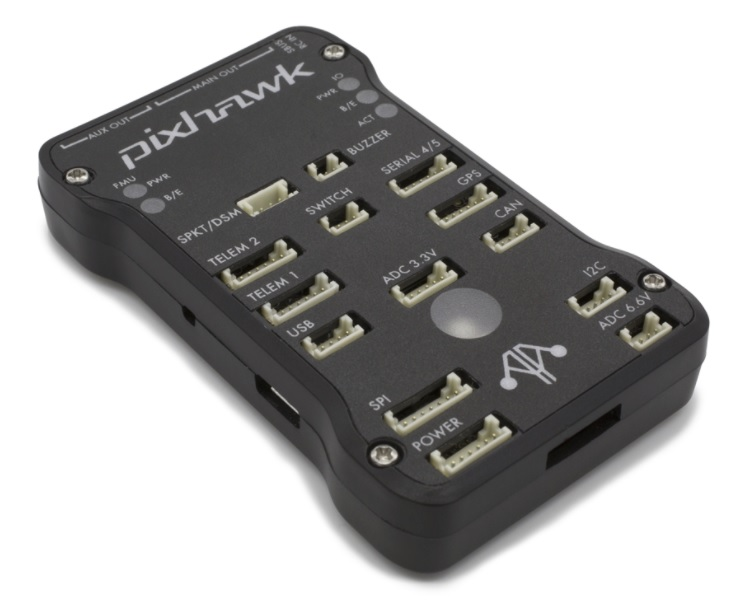
\includegraphics[width=\textwidth]{pixhawk.jpg}
					\caption{"Kontroler" lotu}
				}
			\end{figure}
			\vspace{50pt}
		\end{column}
		\begin{column}{0.72\textwidth}
				\uncover<3->{
					\begin{itemize}
						\item Układ oparty zazwyczaj na~mikrokontrolerze
						\item Posiada wbudowane czujniki, głownie inercyjnie
						\item Prowadzi obliczenia nawigacyjne na podstawie danych z czujników, wyznacza orientację i pozycję 
						\item Stabilizuje i steruje lotem BSP
						\item ...
					\end{itemize}
					\vspace{60pt}
				}
		\end{column}
	\end{columns}
\end{frame}

\begin{frame}
	\frametitle{Motywacja}
	\begin{columns}
		\begin{column}{0.38\textwidth}
			\begin{figure}
				\centering
				\uncover<1->{
					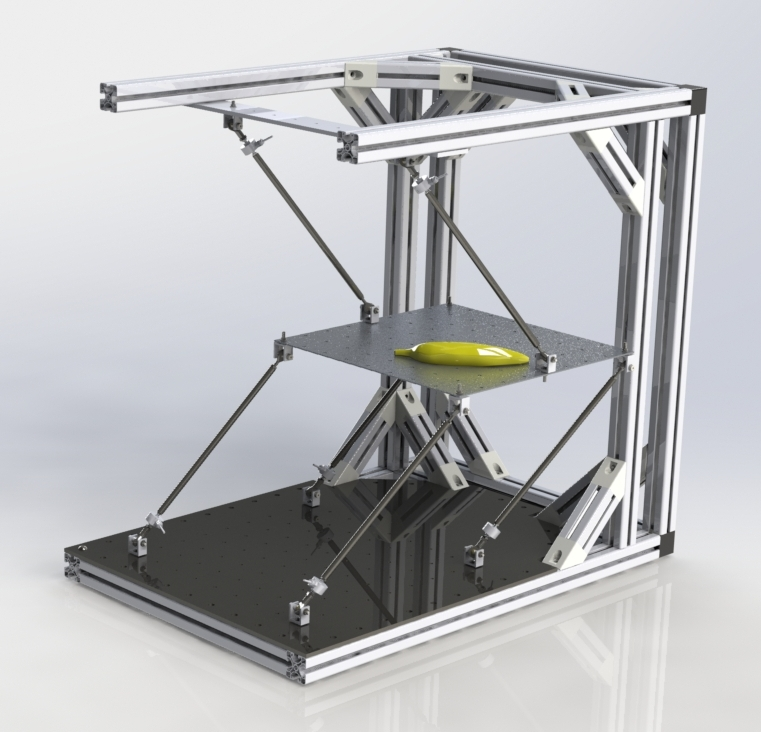
\includegraphics[width=\textwidth]{render.jpg}
					\caption{Układ wieloczłonowy}
				}
			\end{figure}
			\vspace{50pt}
		\end{column}
		\begin{column}{0.72\textwidth}
			\uncover<2->{
				\begin{itemize}
					\item Stanowisko do pomiaru sił reakcji w układach wieloczłonowych z więzami nadmiarowymi
					\item W łącznikach znajdują się liniowe czujniki siły
					\item Ruchoma płyta ma jeden stopień swobody*
					\item Występują dwa punkty bifurkacji
					\item Stanowisko nie posiada czujników pozwalających jego konfigurację
					\item Możliwe jest połączenie układu z robotem przemysłowym
				\end{itemize}
				\vspace{70pt}
			}
		\end{column}
	\end{columns}
\end{frame}

\begin{frame}
	\frametitle{Motywacja}
	\begin{columns}
		\begin{column}{0.4\textwidth}
			\begin{figure}
			\centering
				\uncover<1->{
					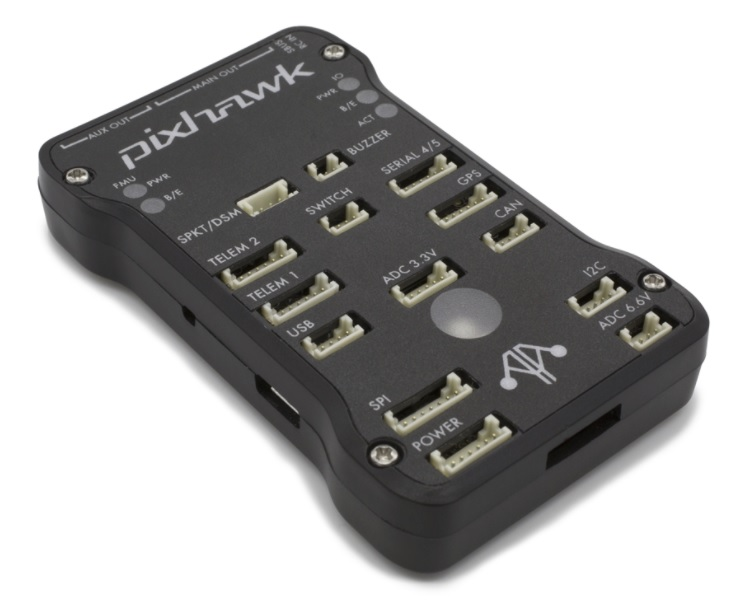
\includegraphics[height=0.62\textheight]{pixhawk.jpg}
					\caption{"Kontroler" lotu}
				}
			\end{figure}
			\vspace{50pt}
		\end{column}
				\begin{column}{0.2\textwidth}
			\begin{figure}
				\centering
				\uncover<1->{
					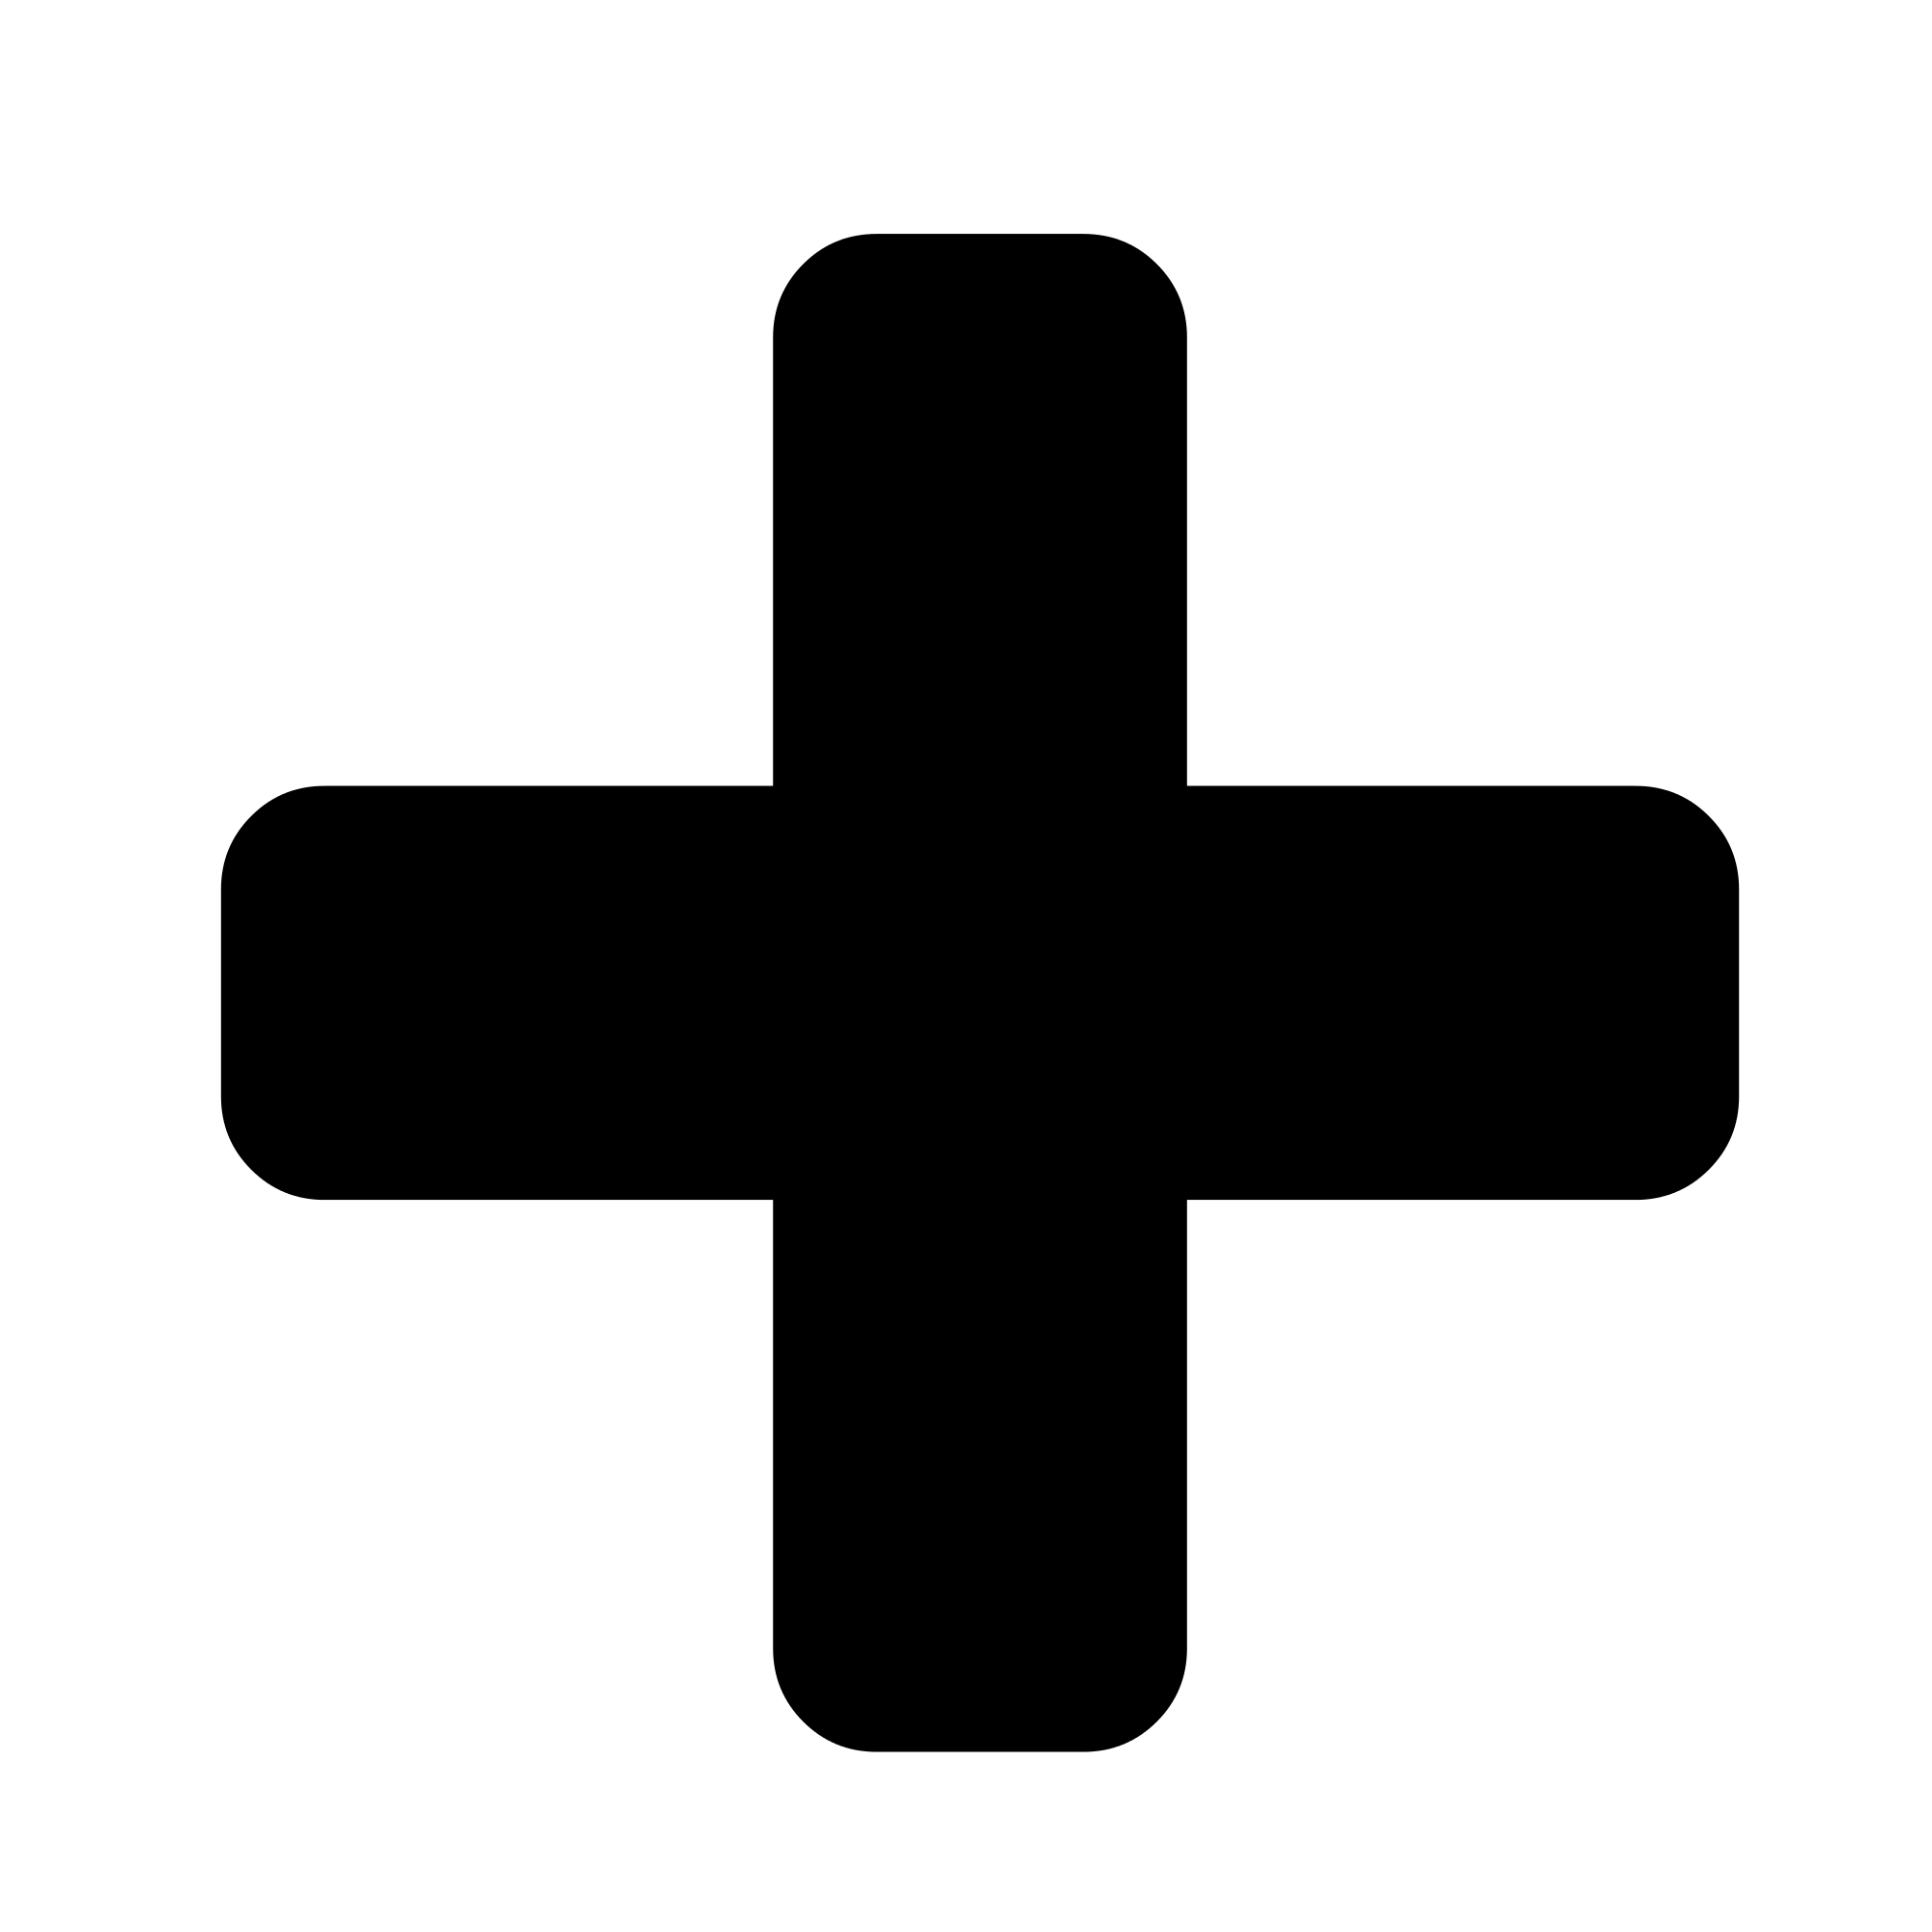
\includegraphics[height=0.2\textheight]{plus.png}
				}
			\end{figure}
			\vspace{50pt}
		\end{column}
		\begin{column}{0.4\textwidth}
			\begin{figure}
				\centering
				\uncover<1->{
					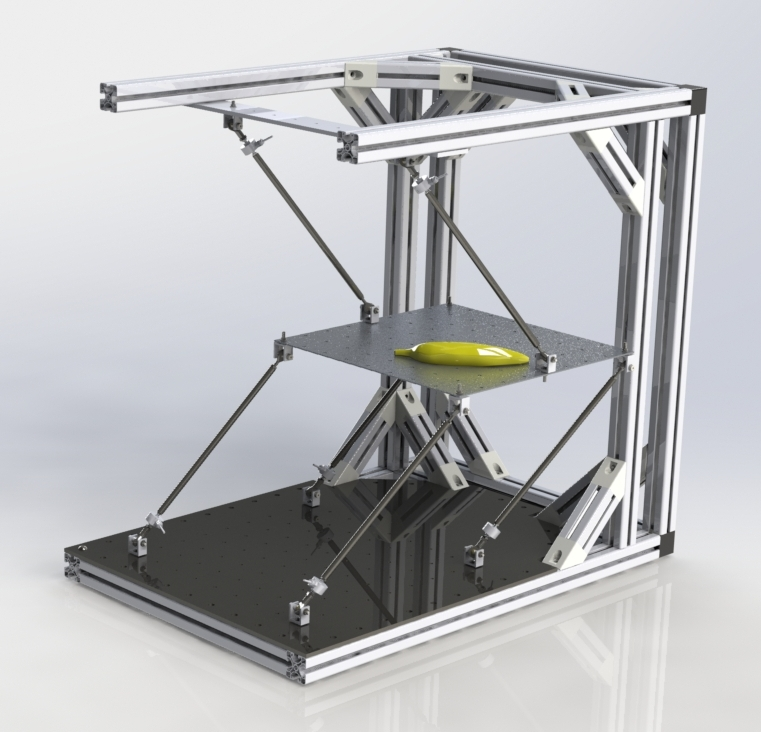
\includegraphics[height=0.65\textheight]{render.jpg}
					\caption{Układ wieloczłonowy}
				}
			\end{figure}
			\vspace{50pt}
		\end{column}
	\end{columns}
\end{frame}

\begin{frame}
	\frametitle{Fazy rozszerzonego filtru Kalmana z korektą więzów}
	\vspace{10pt}
	\begin{center}
		\uncover<1->{
			\begin{tikzpicture}[
				block/.style={rectangle, draw, text width=2cm, text centered, rounded corners, minimum height=1.5cm},
				arrow/.style={->, >=stealth, thick},
				>=Stealth,
				]
				% Nodes
				\node (predict) [block] {Predict};
				\node (correct) [block, right=3cm of predict] {Correction};
				\definecolor{meil_color}{rgb}{0.5,0.5,0.9}
				\node (constraints) [block, fill=meil_color, below left=0.5cm and 0.33cm of correct] {Constraints};
				
				% Arrows
				\draw[arrow] (predict.east)  |- (correct.west) node[midway, above] {};
				\draw[arrow] (correct.south)  |- (constraints.east) node[midway, left] {};
				\draw[arrow] (constraints.west) -- ++(-1.5cm,0) -| (predict.south) node[midway, below] {};
				
			\end{tikzpicture}
		}
	\end{center}
\end{frame}

\begin{frame}
	\frametitle{Cel pracy}
	\begin{itemize}
		\setlength\itemsep{1em}
		\item<1-> Zaadaptowanie nawigacji inercjalnej w systemach określania pozycji i~orientacji robotów.
		\item<1-> Wykorzystanie wiedzy o konstrukcji i istniejących więzach.
		\item<1-> Opracowanie prototypu czujnika i systemu określania pozycji i orientacji.
	\end{itemize}
\end{frame}

\section{Przebieg pracy}

\begin{frame}
	\frametitle{Symulacja komputerowa}	
	\begin{columns}
		\begin{column}{0.4\textwidth}
			\begin{figure}
				\centering
				\uncover<2->{
					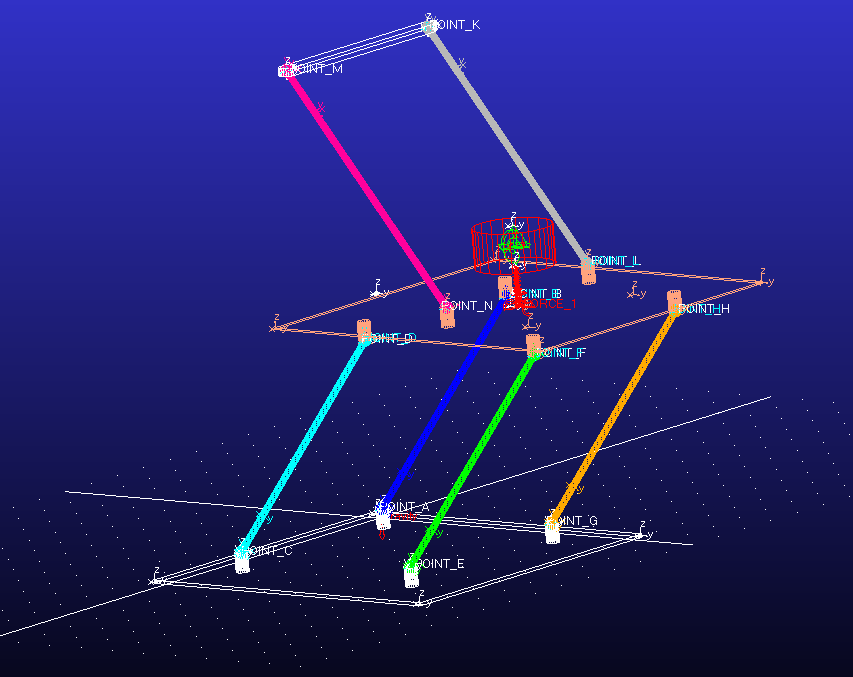
\includegraphics[width=\textwidth]{duw/adams.png}
					\caption{Model stanowiska w ADAMS}
				}
			\end{figure}
			\vspace{50pt}
		\end{column}
		\begin{column}{0.6\textwidth}
			\begin{figure}
				\centering
				\uncover<3->{
					\vspace{15pt}
					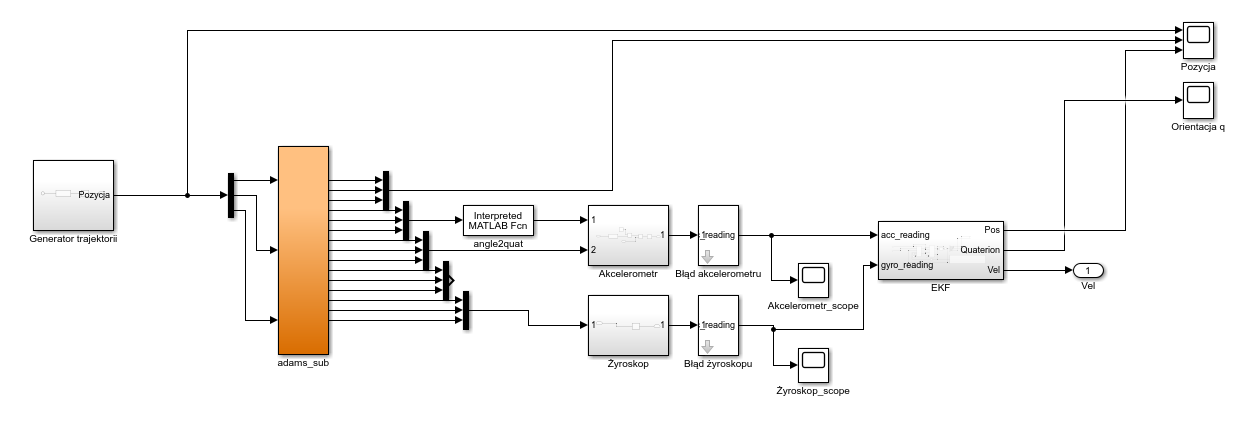
\includegraphics[width=\textwidth]{duw/sys.png}
					\vspace{13pt}
					\caption{System określania pozycji w MATLAB Simulink}
				}
			\end{figure}
			\vspace{50pt}
		\end{column}
	\end{columns}
\end{frame}

\begin{frame}
	\frametitle{Symulacja komputerowa -- wyniki}	
	\begin{columns}
		\begin{column}{0.5\textwidth}
			\begin{figure}
				\centering
				\uncover<1->{
					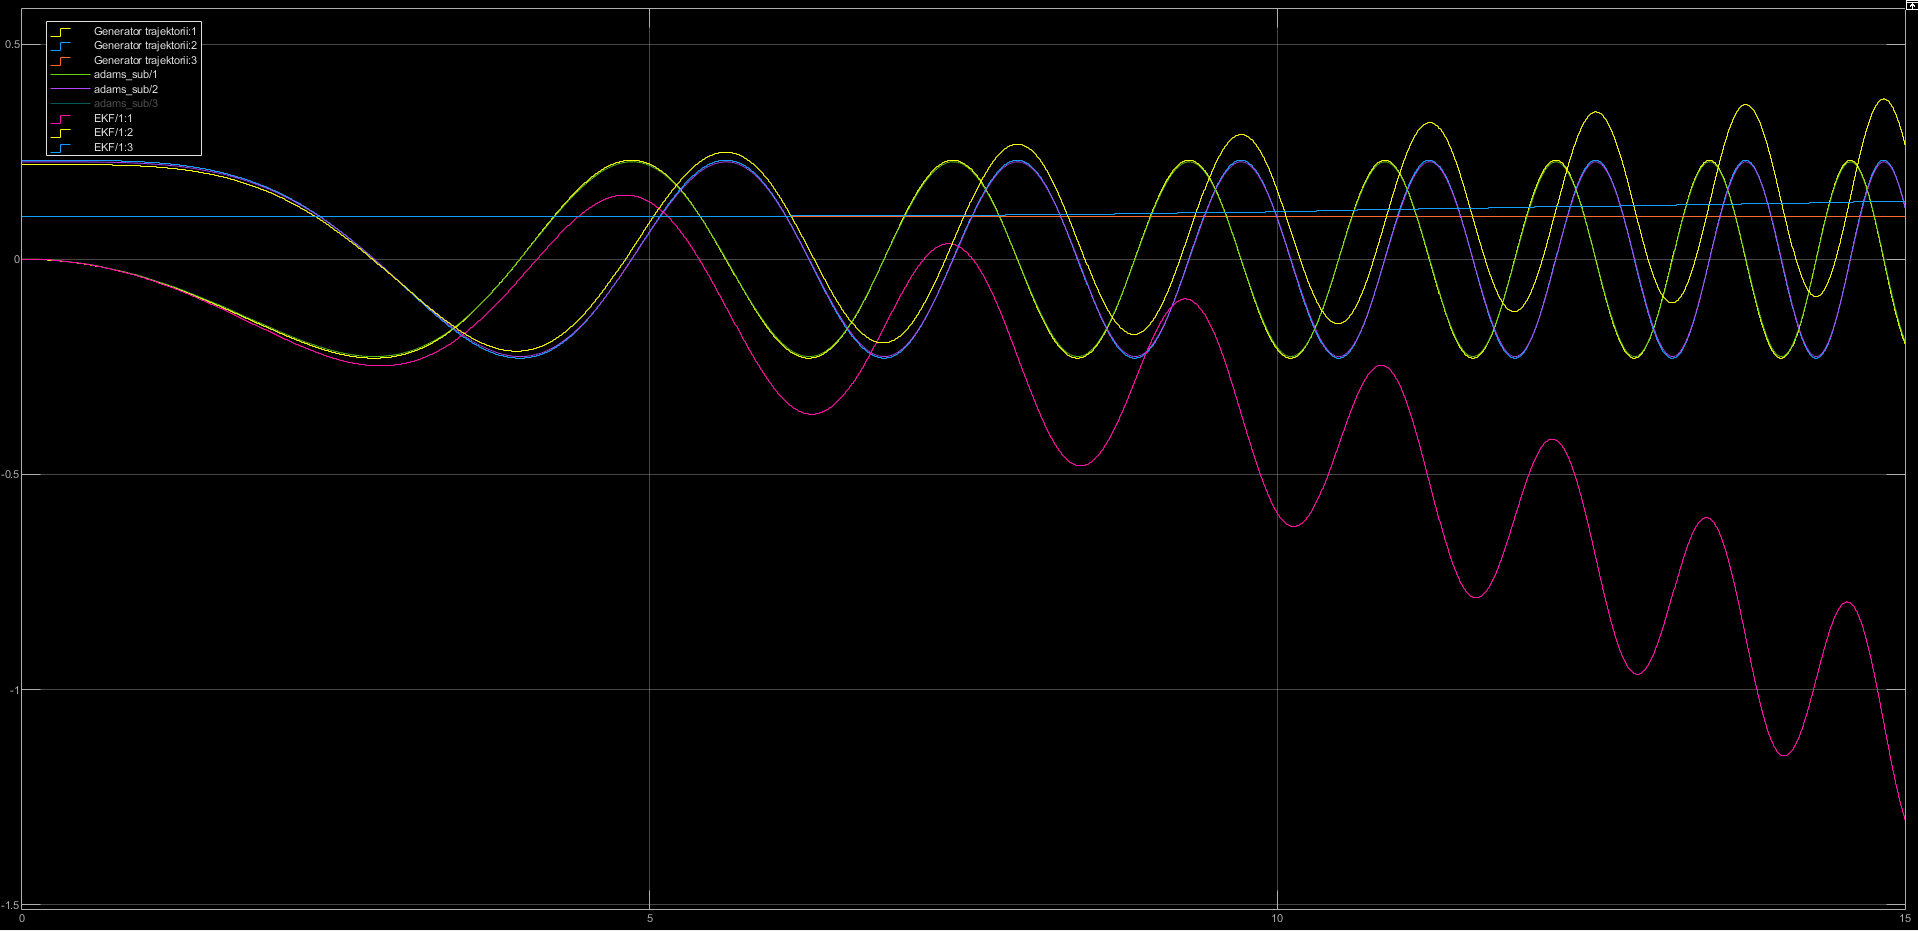
\includegraphics[width=\textwidth]{duw/no_con.png}
					\caption{Symulacja -- brak korekty}
				}
			\end{figure}
		\end{column}
		\begin{column}{0.5\textwidth}
			\begin{figure}
				\centering
				\uncover<1->{
					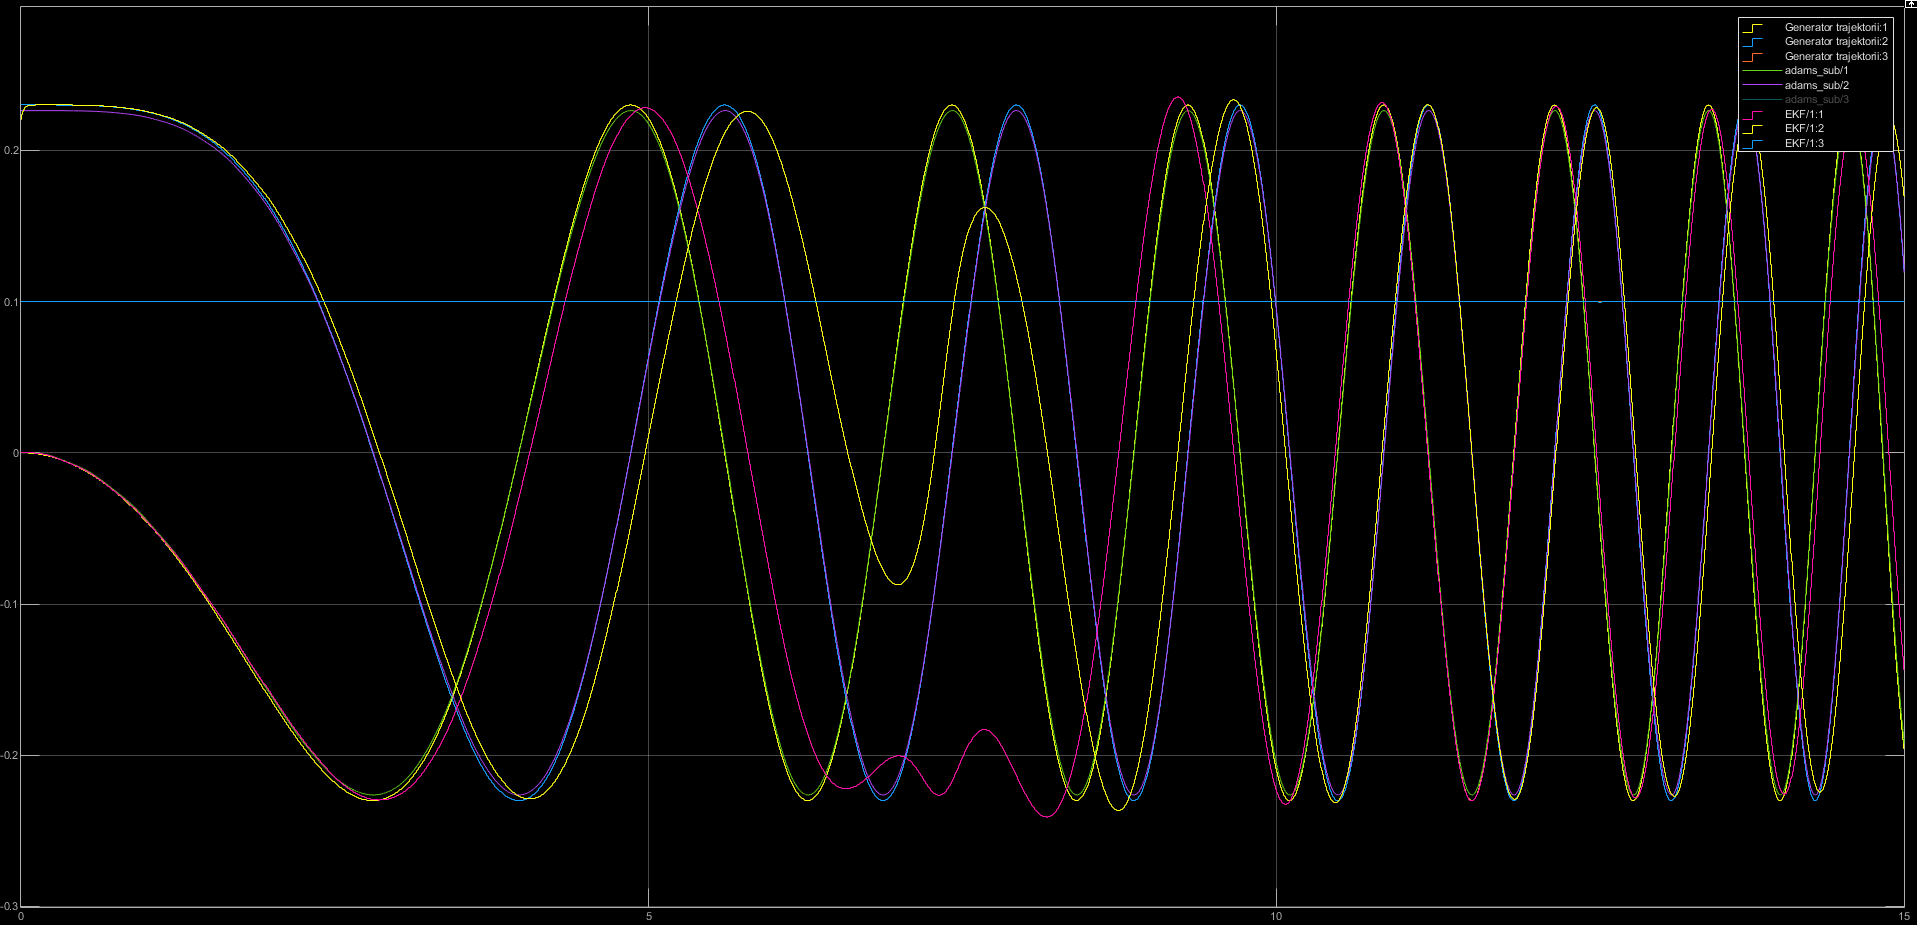
\includegraphics[width=\textwidth]{duw/corr.png}
					\caption{Symulacja -- z korektą}
				}
			\end{figure}
		\end{column}
	\end{columns}
\end{frame}

\begin{frame}
	\frametitle{Rozszerzony  przegląd stanu wiedzy}	
	\begin{itemize}
		\item<1-> modele matematyczne czujników, modelowanie błędu pomiarowego
		\item<1-> metody filtracji danych i kalibracji czujników
		\item<1-> metody fuzji danych
		\item<1-> problem synchronizacji czasu, problem przesyłu danych pomiarowych
		\item<1-> więzy w układach wieloczłonowych
	\end{itemize}
\end{frame}

\begin{frame}
	\frametitle{Budowa prototypu zintegrowanego czujnika}
	\begin{columns}
		\begin{column}{0.5\textwidth}
			\begin{figure}
				\centering
				\uncover<1->{
					\vspace{15pt}
					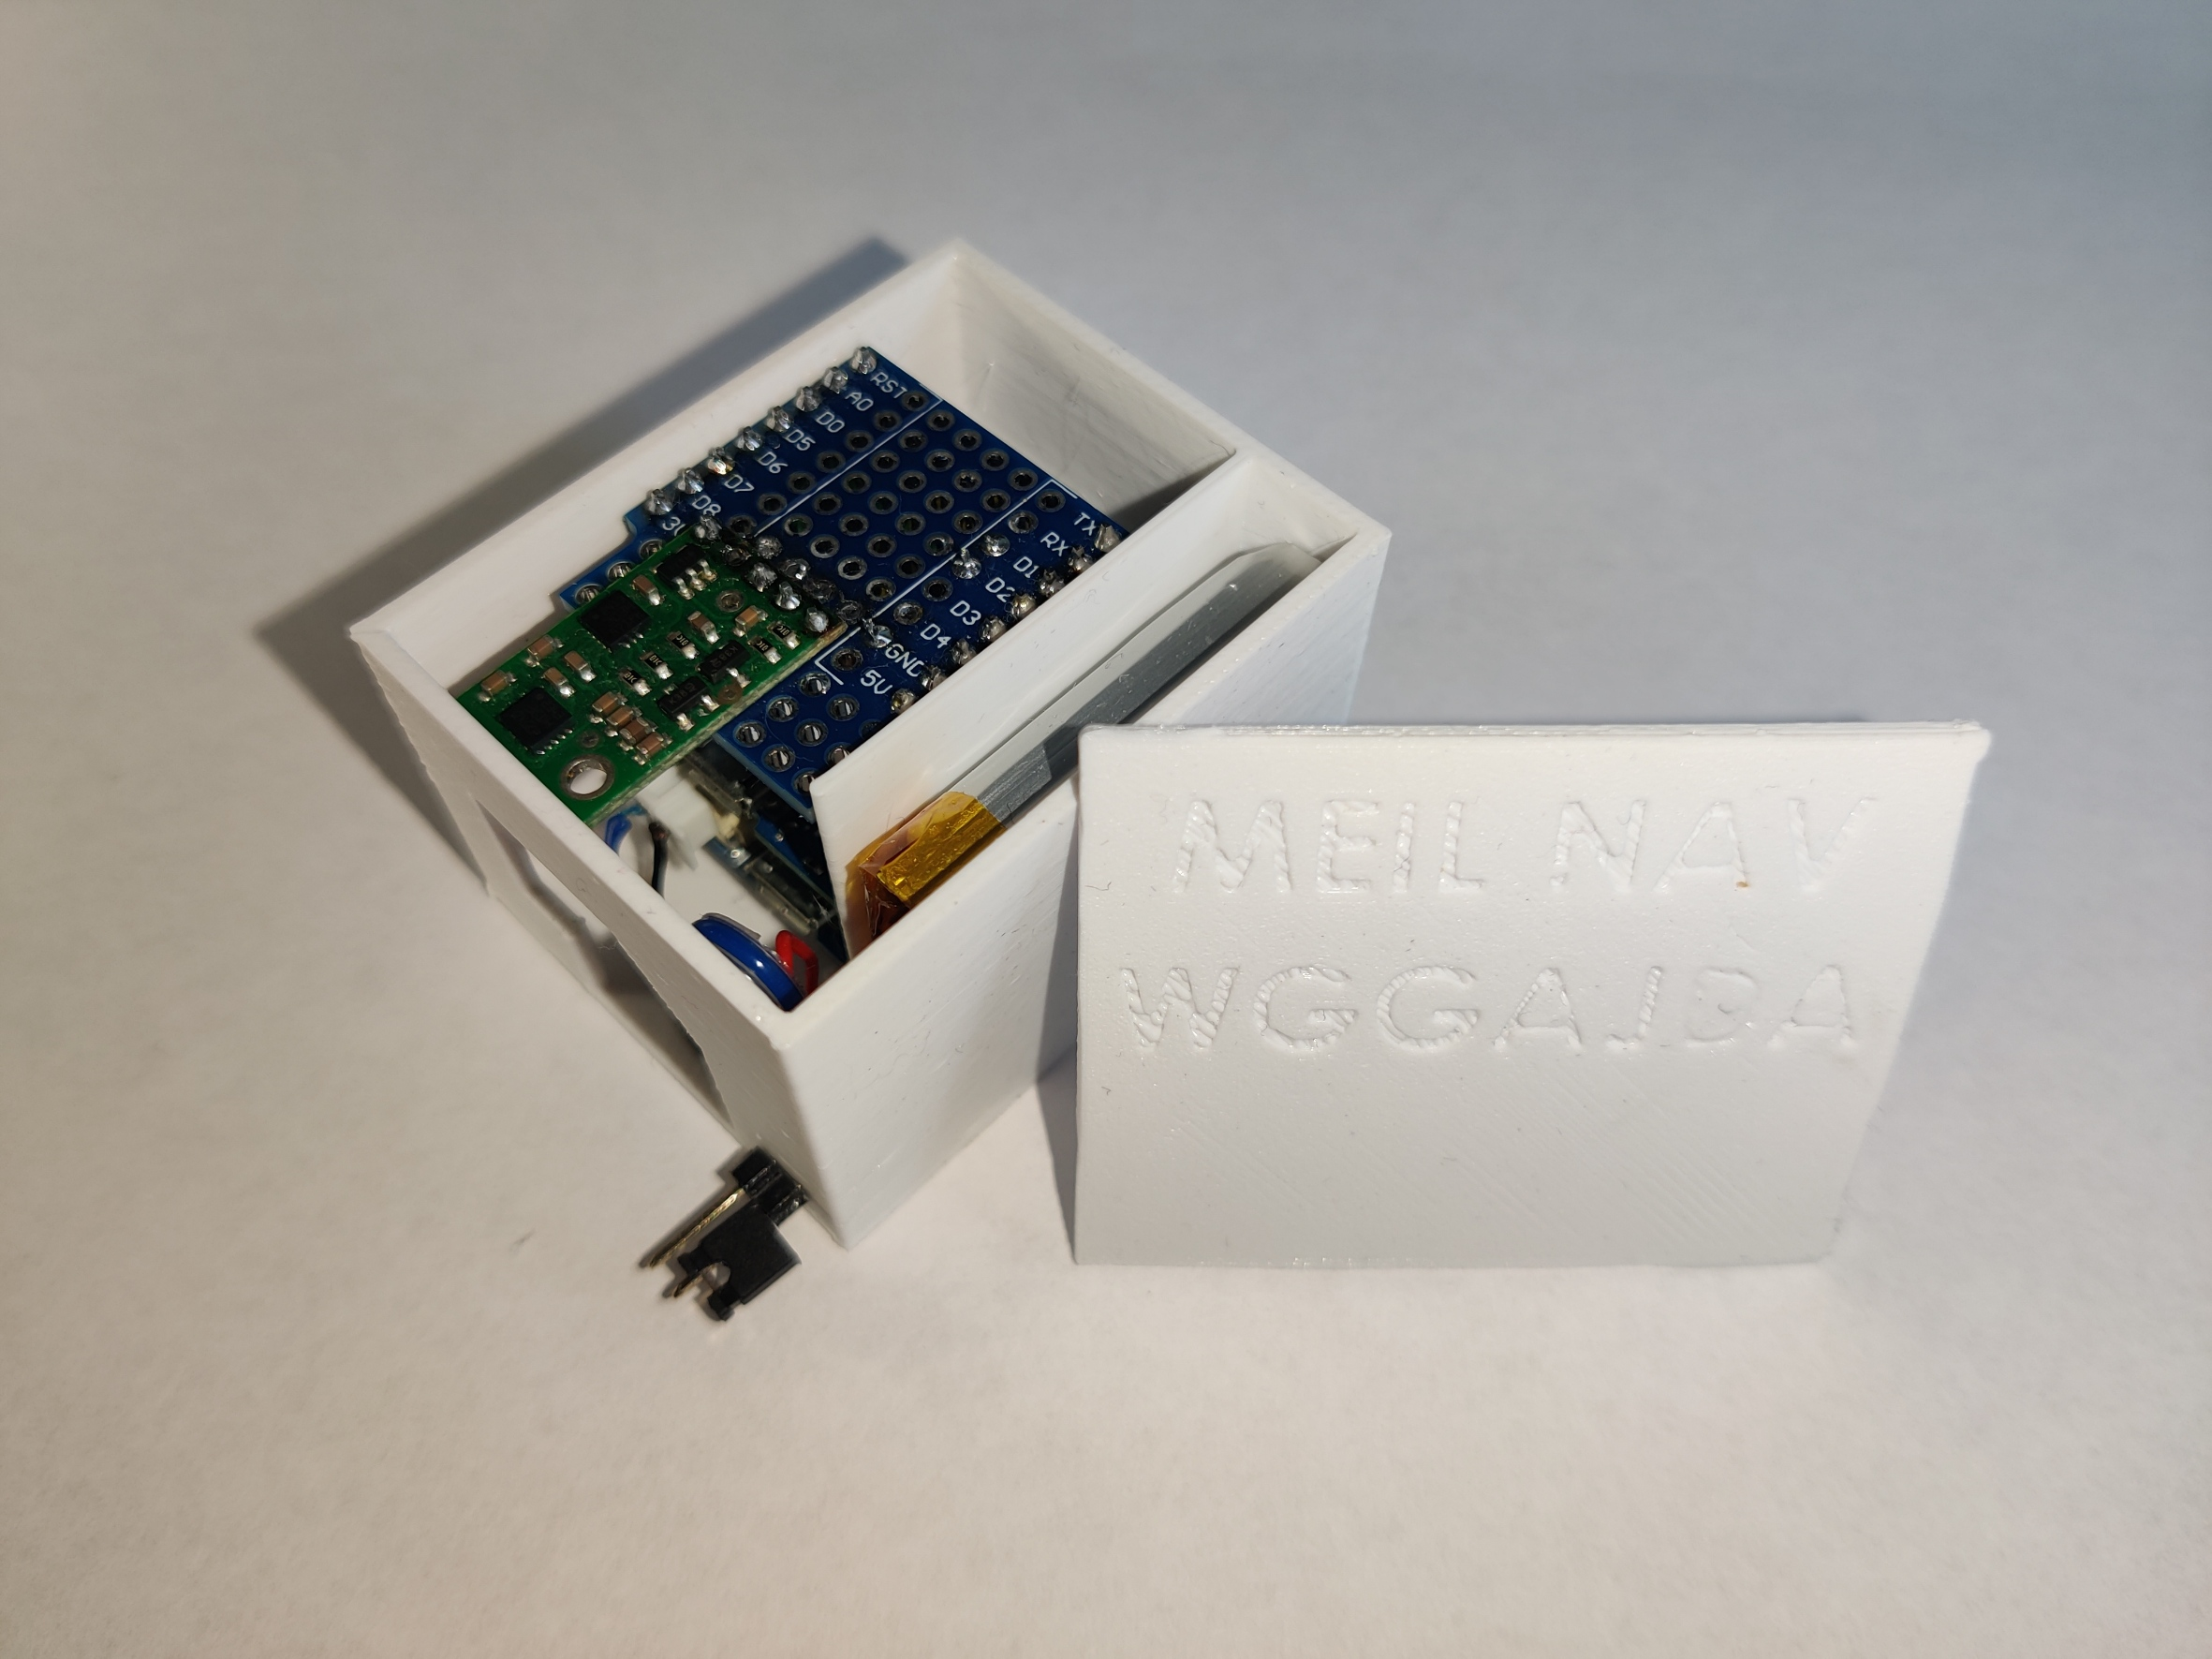
\includegraphics[width=0.9\textwidth]{prototype.jpg}
					\caption{Prototyp}
				}
			\end{figure}
			\vspace{50pt}
		\end{column}
		\begin{column}{0.72\textwidth}
			\uncover<2->{
				\begin{itemize}
					\item Oparty na mikrokontrolerze EPS32
					\item Posiada akcelerometr, żyroskop i magnetometr
					\item Zasilany bateryjne
					\item Przesyła surowe dane z wykorzystaniem UDP
					\item Częstotliwość próbkowania wynosi \textasciitilde 500Hz
				\end{itemize}
				\vspace{80pt}
			}
		\end{column}
	\end{columns}
\end{frame}


\begin{frame}
	\frametitle{Architektura systemu}
	\begin{figure}
		\centering
		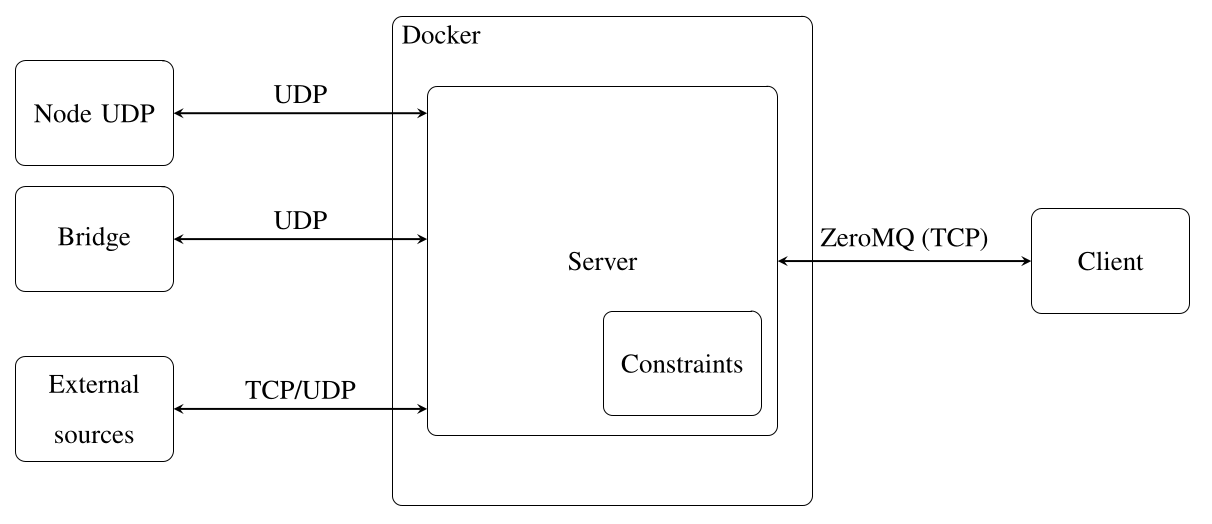
\includegraphics[width=1\textwidth]{arch.png}
		%\caption{Prototyp zintegrowanego czujnika inercyjnego}
	\end{figure}
\end{frame}

\begin{frame}
	\frametitle{Dobór  technologii}
	\begin{columns}
		\begin{column}{0.33\textwidth}
			\begin{figure}
				\centering
				\uncover<1->{
\includegraphics[height=0.2\textheight]{logos/cpp.png}}
			\end{figure}
			\begin{figure}
				\centering
				\uncover<1->{
\includegraphics[height=0.2\textheight]{logos/eigen.png}}
			\end{figure}
		\end{column}
		\begin{column}{0.33\textwidth}
			\begin{figure}
				\centering
				\uncover<1->{
\includegraphics[height=0.2\textheight]{logos/python.png}}
			\end{figure}
			\begin{figure}
				\centering
				\uncover<1->{
\includegraphics[height=0.2\textheight]{logos/Qt.png}}
			\end{figure}
		\end{column}
		\begin{column}{0.33\textwidth}
			\begin{figure}
				\centering
				\uncover<1->{
\includegraphics[height=0.2\textheight]{logos/matlab.png}}
			\end{figure}
			\begin{figure}
				\centering
				\uncover<1->{
\includegraphics[height=0.2\textheight]{logos/docker.png}}
			\end{figure}
		\end{column}
	\end{columns}
\end{frame}

\begin{frame}
	\frametitle{Graficzny interfejs użytkownika I}
	\begin{figure}
		\centering
		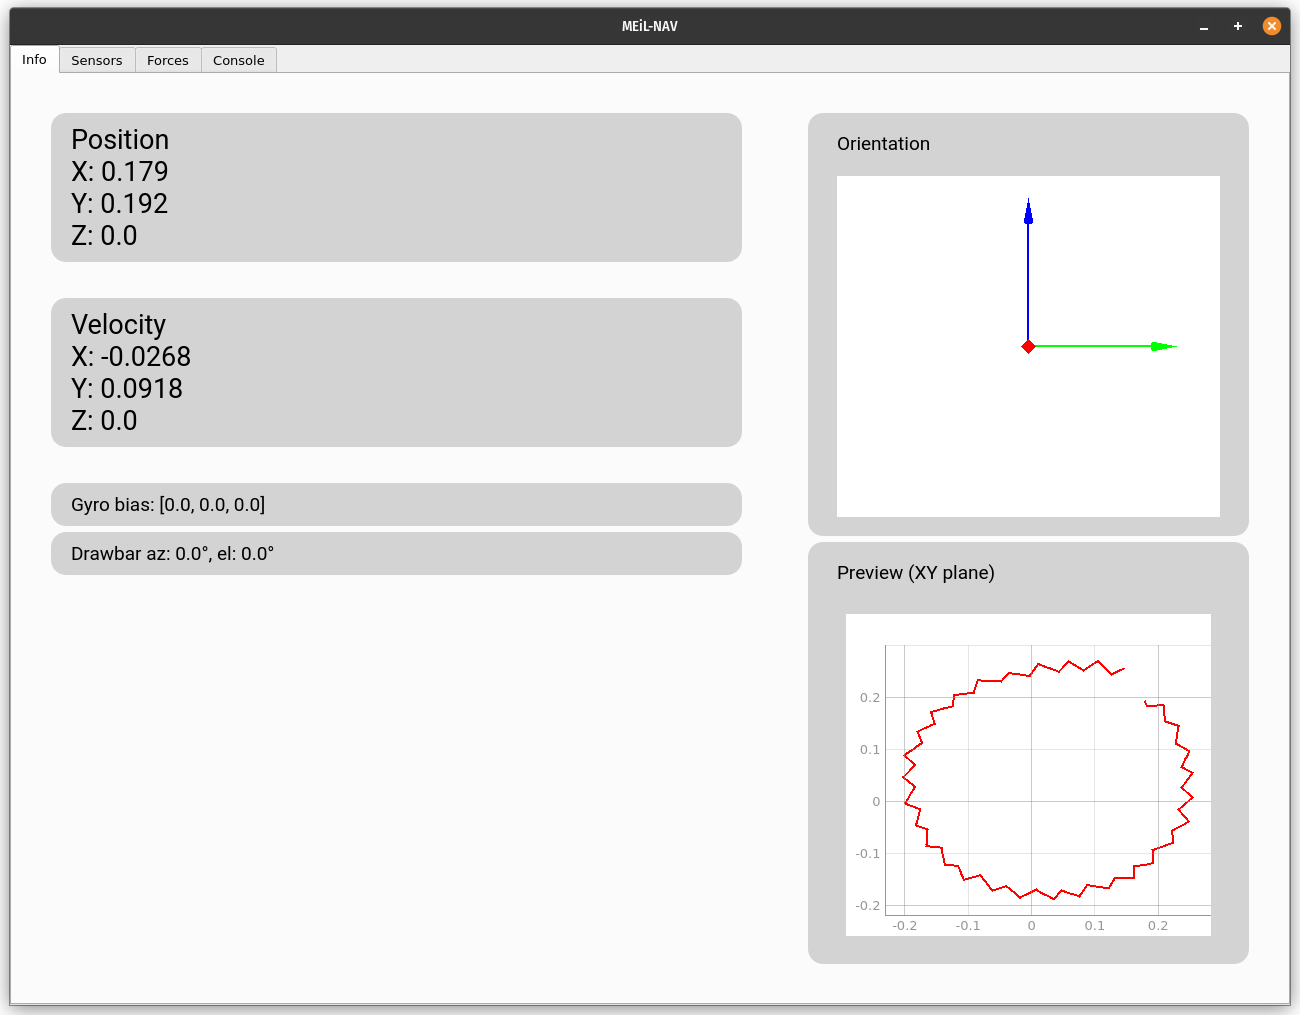
\includegraphics[width=0.6\textwidth]{gui_dashboard.png}
		\caption{Zakładka \textit{Info}}
	\end{figure}
\end{frame}

\begin{frame}
	\frametitle{Graficzny interfejs użytkownika II}
	\begin{figure}
		\centering
		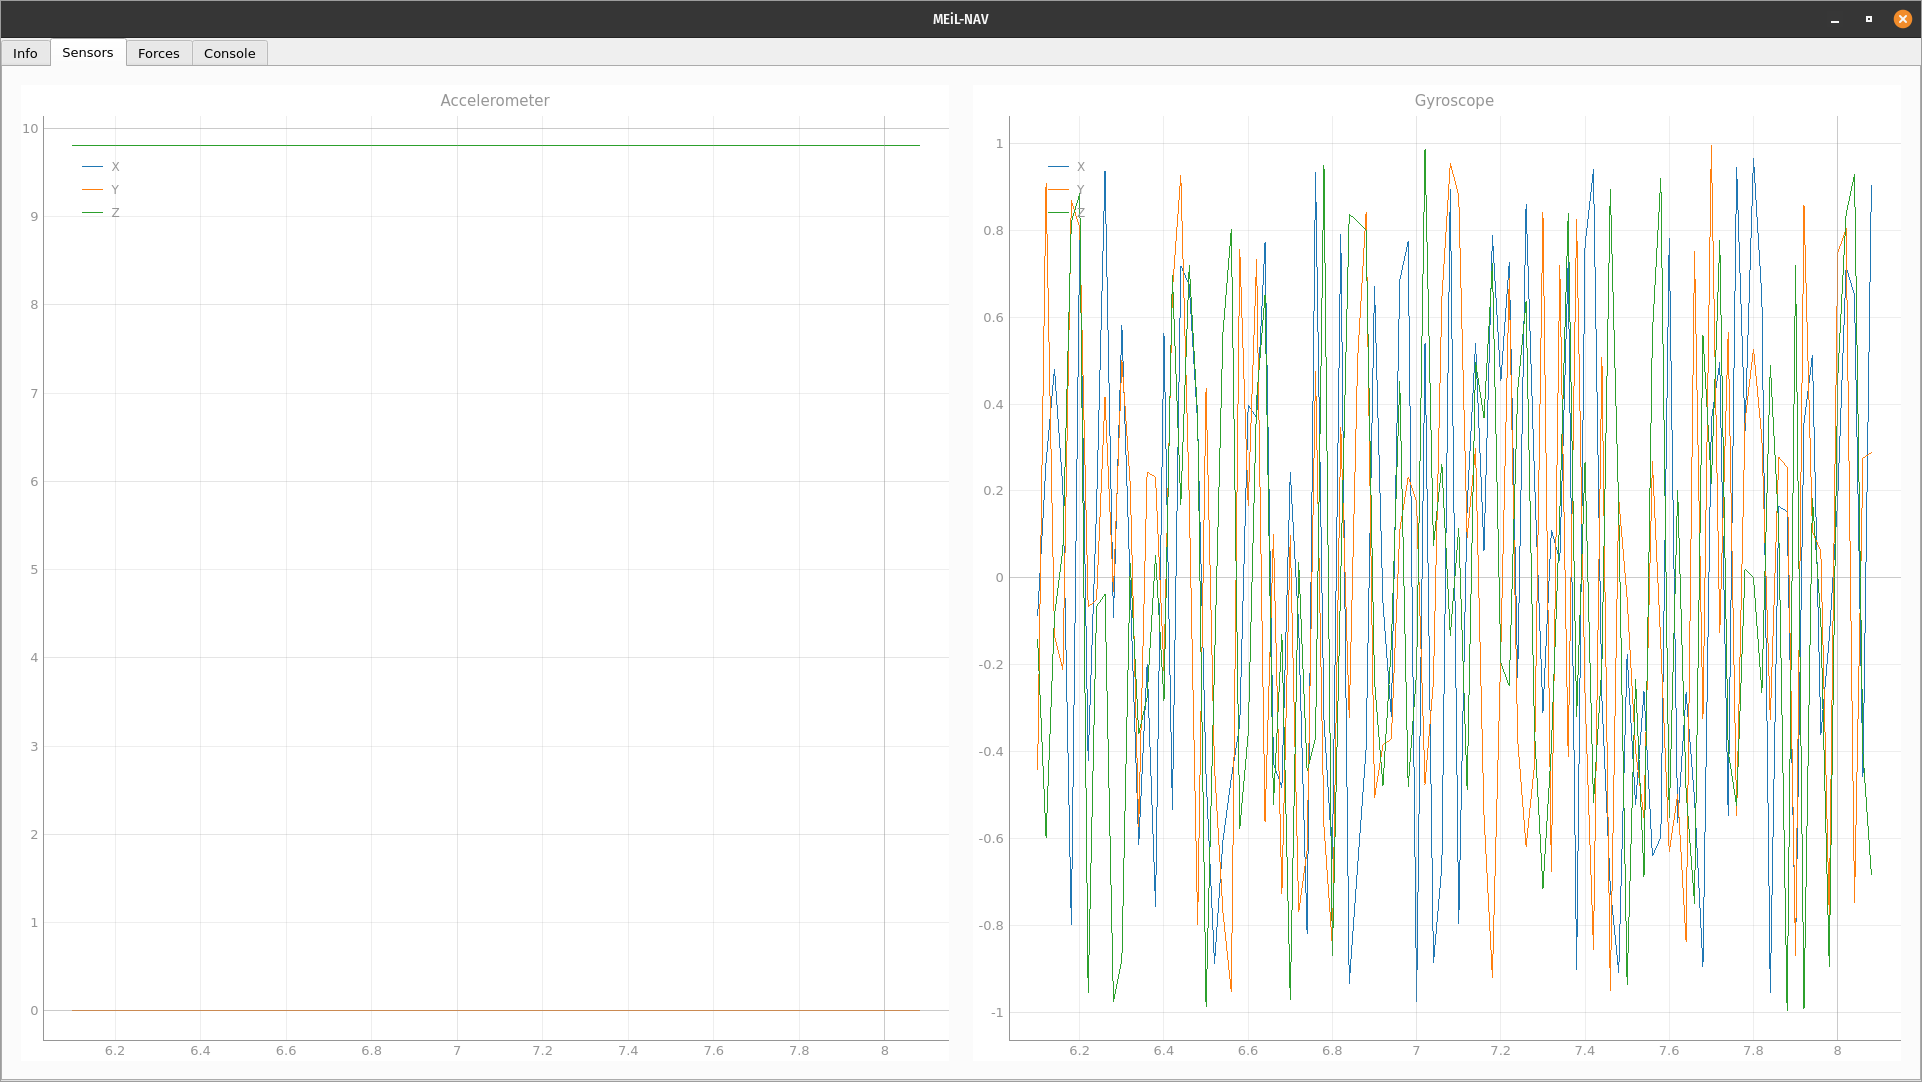
\includegraphics[width=0.7\textwidth]{gui_sensor.png}
		\caption{Zakładka \textit{Sensors}}
	\end{figure}
\end{frame}

\begin{frame}
	\frametitle{Graficzny interfejs użytkownika III}
	\begin{figure}
		\centering
		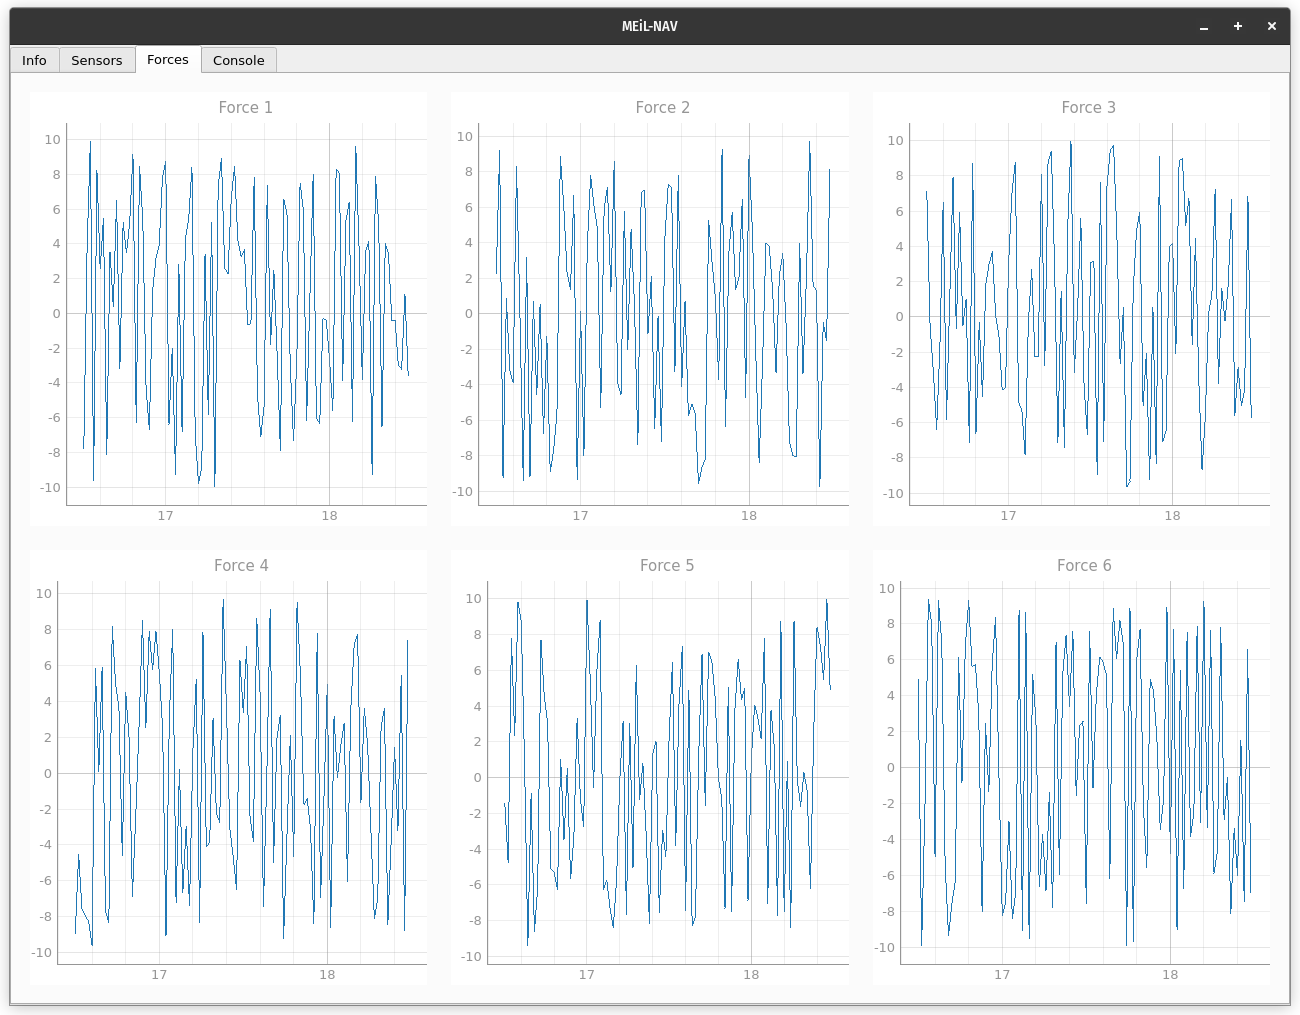
\includegraphics[width=0.6\textwidth]{gui_force.png}
		\caption{Zakładka \textit{Forces}}
	\end{figure}
\end{frame}

\begin{frame}
	\frametitle{Graficzny interfejs użytkownika IV}
	\begin{figure}
		\centering
		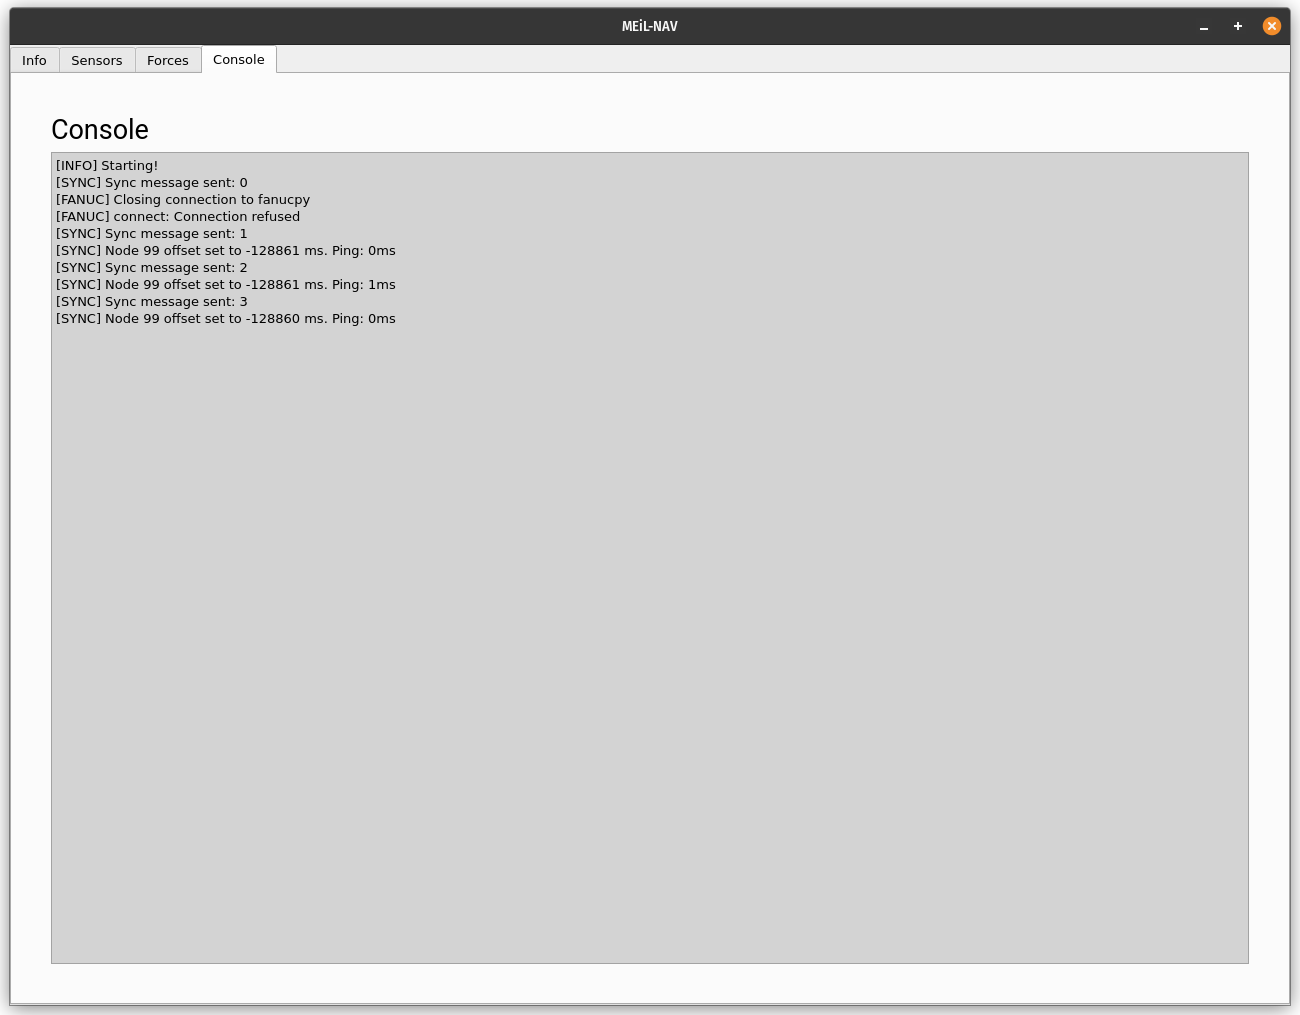
\includegraphics[width=0.6\textwidth]{gui_consol.png}
		\caption{Zakładka \textit{Console}}
	\end{figure}
\end{frame}

\begin{frame}
	\frametitle{Pomiary}
	\begin{figure}
		\centering
		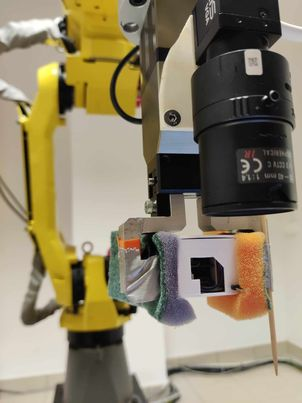
\includegraphics[width=0.35\textwidth]{sensor_mount.jpg}
		\caption{Czujnik  zamontowany  na robocie  FANUC}
	\end{figure}
\end{frame}

\begin{frame}
	\frametitle{Pomiary -- określenie orientacji robota \href{run:attitude_test.mp4}{\beamergotobutton{Film}}}
	\begin{columns}
		\begin{column}{0.5\textwidth}
			
			\begin{figure}
				\centering
				\uncover<2->{
					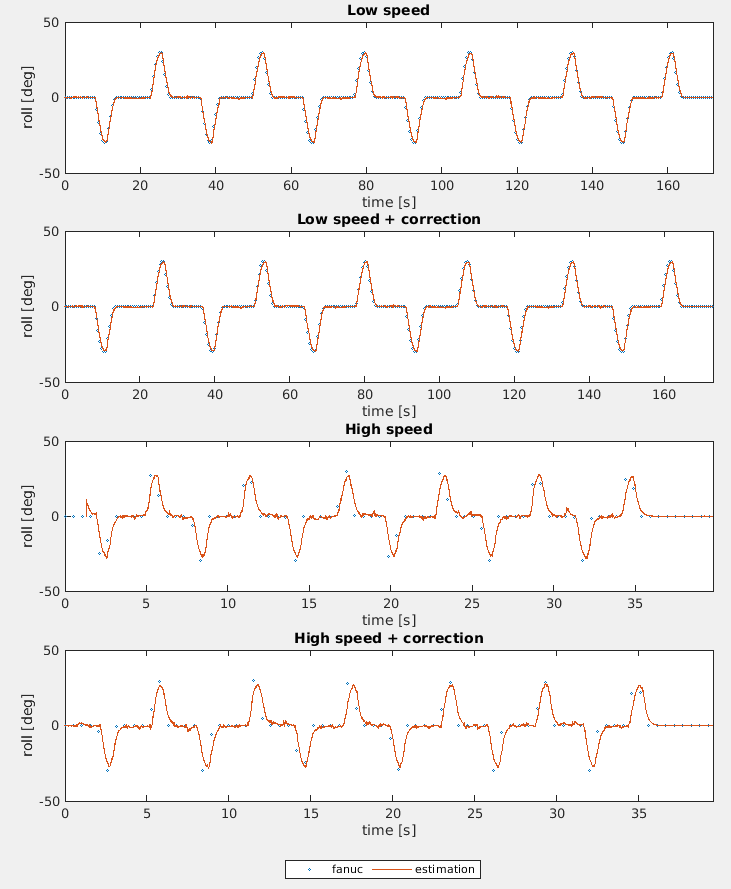
\includegraphics[height=0.77\textheight]{ori_est_roll.png}
					\caption{Kąt przechylenia}
				}
			\end{figure}
		\end{column}
		\begin{column}{0.5\textwidth}
			\begin{figure}
				\centering
				\uncover<2->{
					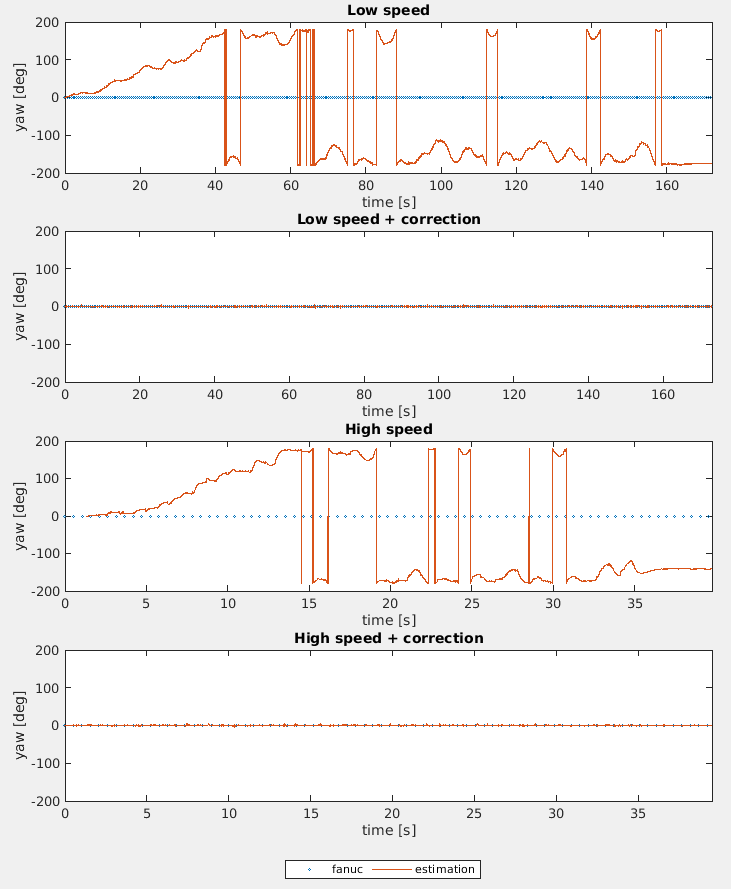
\includegraphics[height=0.77\textheight]{ori_est_yaw.png}
					\caption{Kąt odchylenia}
				}
			\end{figure}
		\end{column}
	\end{columns}
\end{frame}

\begin{frame}
	\frametitle{Pomiary -- określenie pozycji robota \href{run:position_test.mp4}{\beamergotobutton{Film}}}
	\begin{columns}
		\begin{column}{0.5\textwidth}
			\begin{figure}
				\centering
				\uncover<2->{
					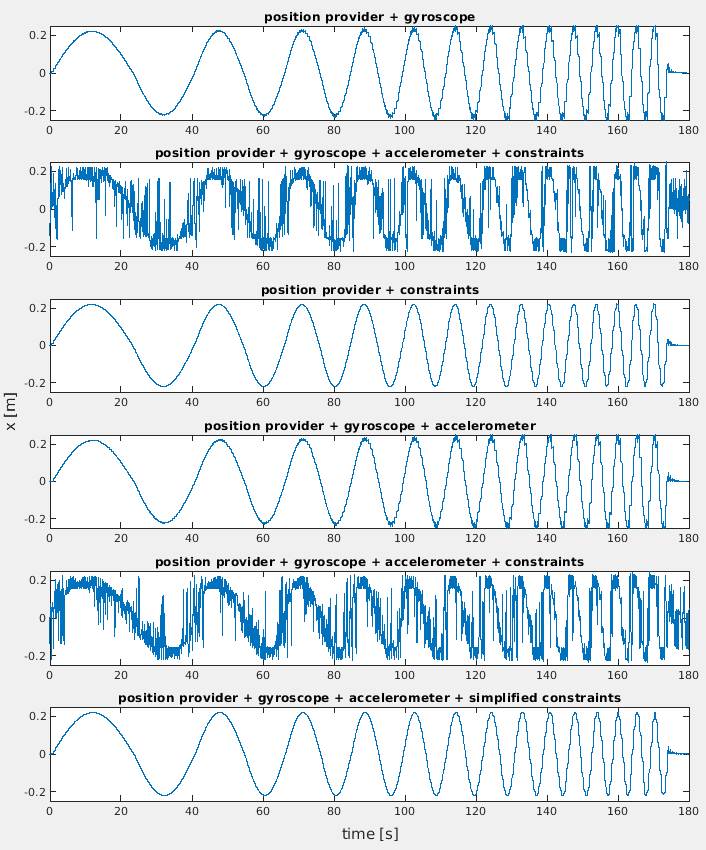
\includegraphics[height=0.77\textheight]{pos_est_x.png}
					\caption{Przemieszczenie  x}
				}
			\end{figure}
		\end{column}
		\begin{column}{0.5\textwidth}
			\begin{figure}
				\centering
				\uncover<2->{
					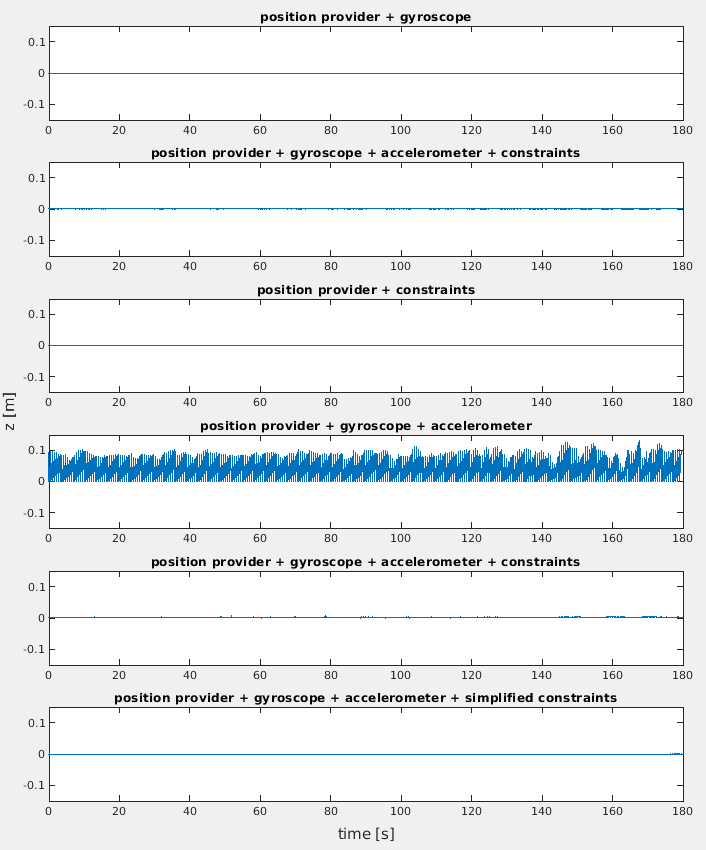
\includegraphics[height=0.77\textheight]{pos_est_z.png}
					\caption{Przemieszczenie  z}
				}
			\end{figure}
		\end{column}
	\end{columns}
\end{frame}

\section{Podsumowanie}

\begin{frame}
	\frametitle{Podsumowanie}	
	\uncover<1->{W ramach pracy udało się:}
	\begin{itemize}
		\item<1-> dokonać rozległego przeglądu stanu wiedzy,
		\item<1-> opracować model filtru Kalmana uwzględniający więzy,
		\item<1-> zbudować prototyp zintegrowanego czujnika,
		\item<1-> opracować system umożliwiający określenie pozycji i orientacji robota.
	\end{itemize}
\end{frame}

\begin{frame}{References}
	\frametitle{Bibliografia (wybrane pozycje)}
	\begin{thebibliography}{10}
		\beamertemplatebookbibitems
		\bibitem{simon}[2002] Kalman filtering with state equality constraints
		\newblock Simon, D. and Tien Li Chia
		\bibitem{farrell}[2012] Integrated Aircraft Navigation
		\newblock Farrell, J.
		\bibitem{joint}[2012] Joint reactions in rigid or flexible body mechanisms with redundant constraints
		\newblock Wojtyra, Marek and Frączek, Janusz
		\bibitem{more} ... i 33 inne publikacje zawarte w pracy.
	\end{thebibliography}
\end{frame}

\begin{frame}
	  \begin{center}
	\Huge Dziękuje za uwagę!
	\end{center}
\end{frame}

\end{document}